\chapter{Cuidar da natureza}\label{ch:g2:caring-for-nature}

Depois do piquenique, uma família deixa o campo exatamente como
encontrou; outra deixa sacolas, tampinhas de garrafa e um
formigueiro pisoteado. Os coelhos, as formigas e as margaridas do
campo não conseguem pedir que a gente tome cuidado --- mas são \omterm{def:g1:living-or-not:living}{seres
vivos} dividindo os nossos lugares, e o nosso jeito de agir na
\omterm{def:g2:caring-for-nature:environment}{natureza} faz diferença para eles. Cuidar da \omterm{def:g2:caring-for-nature:environment}{natureza} é algo que
qualquer pessoa pode aprender, em qualquer idade.

\section{A natureza é onde os seres vivos vivem}

\begin{definition}[Natureza e ambiente]\label{def:g2:caring-for-nature:environment}
A \emph{natureza}\index{natureza} é o mundo dos \omterm{def:g1:living-or-not:living}{seres vivos} e do que
está em volta deles: campos, florestas, lagoas, mares --- e o ar, a
água e o solo de que eles dependem. Aquilo que está em volta de um
\omterm{def:g1:living-or-not:living}{ser vivo} e do que ele depende se chama \emph{ambiente}\index{ambiente}.
\end{definition}

\begin{example}[Tudo é a casa de alguém]\label{ex:g2:caring-for-nature:home}
Um tronco apodrecido na floresta parece lixo --- e é um palácio:
besouros debaixo da casca, tatuzinhos por baixo, musgo em cima, um
ouriço passando o inverno no oco. Chute o tronco por brincadeira e
quatro famílias perdem a casa. Na \omterm{def:g2:caring-for-nature:environment}{natureza}, quase tudo é a casa, o
alimento ou o abrigo de alguém.
\end{example}

\begin{omfigure}
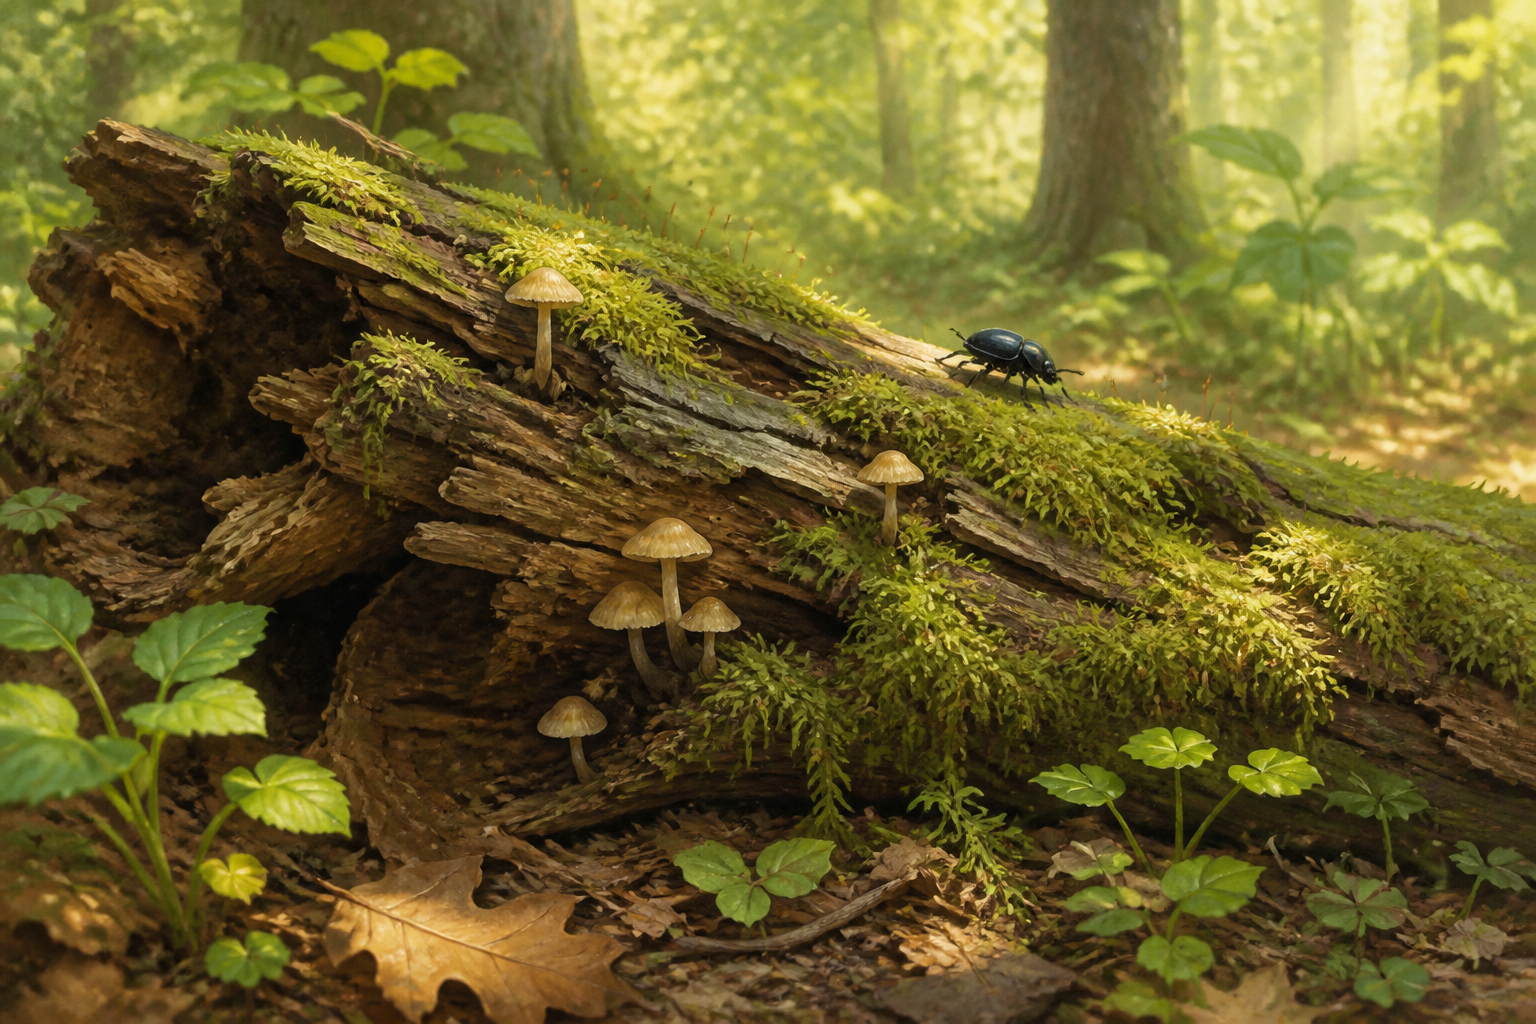
\includegraphics[width=0.62\linewidth]{images/book1/ai/g2-nature-log.png}

{\small O tronco apodrecido que na verdade é um palácio: musgo no
telhado, cogumelos nas paredes, um besouro no corredor.}
\end{omfigure}

\begin{remark}[Nós fazemos parte disso]\label{rem:g2:caring-for-nature:part}
As pessoas também são \omterm{def:g1:living-or-not:living}{seres vivos}: o ar que respiramos, a água que
bebemos e o alimento que comemos vêm todos da \omterm{def:g2:caring-for-nature:environment}{natureza}. Cuidar dela
não é só gentileza com os coelhos --- é cuidar do mundo do qual nós
mesmos vivemos, como o \cref{ch:g2:where-animals-live} disse de todo
\omterm{def:g2:where-animals-live:habitat}{hábitat}.
\end{remark}

\section{O que faz mal, o que ajuda}

\begin{proposition}[Ações pequenas, danos de verdade]\label{prop:g2:caring-for-nature:harm}
Na \omterm{def:g2:caring-for-nature:environment}{natureza}, o dano quase nunca vem da vontade de fazer o mal ---
vem de não pensar:
\begin{itemize}
  \item o lixo fica ali por anos e pode prender ou envenenar
        \omterm{def:g1:animals-around-us:animal}{animais};
  \item colher todas as \omterm{def:g1:plants-around-us:parts}{flores} não deixa nenhuma para fazer
        \omterm{def:g2:from-seed-to-plant:seed}{sementes} --- e nenhuma para as abelhas;
  \item gritaria e correria atrás dos bichos afastam os \omterm{def:g1:animals-around-us:animal}{animais} do
        alimento e dos filhotes deles;
  \item margens pisoteadas, pedras viradas e \omterm{def:g1:plants-around-us:tree}{galhos} quebrados
        desfazem, cada um, uma casinha.
\end{itemize}
\end{proposition}
\admitted

\begin{example}[A tampinha de garrafa]\label{ex:g2:caring-for-nature:cap}
Uma tampinha de plástico jogada no chão não é nada para nós e fica
no campo por muitos e muitos anos --- tempo suficiente para os
adultos terem filhos que acham a mesma tampinha. A \omterm{def:g2:caring-for-nature:environment}{natureza} não tem
caminhão de lixo: o que a gente deixa, fica.
\end{example}

\begin{method}[As regras do visitante]\label{met:g2:caring-for-nature:rules}
Lá fora, na \omterm{def:g2:caring-for-nature:environment}{natureza}:
\begin{enumerate}
  \item leve todo o seu lixo para casa --- todo ele;
  \item olhe as \omterm{def:g1:plants-around-us:parts}{flores}, os insetos e os ninhos em vez de coletar;
        colha no máximo algumas \omterm{def:g1:plants-around-us:parts}{flores} comuns, nunca um tufo
        inteiro;
  \item recoloque cada pedra e cada tronco que você virar ---
        alguém mora embaixo;
  \item fique nas trilhas perto de lugares frágeis, como as margens
        dos riachos;
  \item observe os \omterm{def:g1:animals-around-us:animal}{animais} de longe, em silêncio, e não mexa nos
        filhotes deles.
\end{enumerate}
Deixe o lugar de um jeito que ninguém consiga dizer que você esteve lá.
\end{method}

\begin{example}[Ajudar de propósito]\label{ex:g2:caring-for-nature:help}
Cuidar pode ir além de não fazer mal. Um pratinho de água numa onda
de calor, um cantinho selvagem do quintal deixado sem cortar,
\omterm{def:g2:from-seed-to-plant:seed}{sementes} para as aves no frio, uma lagoa de escola como a do
\cref{ex:g2:where-animals-live:schoolpond}: cada uma dessas coisas
dá a alguns \omterm{def:g1:living-or-not:living}{seres vivos} o alimento, a água ou a casa que eles tinham
perdido.
\end{example}

\section{Separar e economizar}

\begin{proposition}[O lixo pode ser devolvido]\label{prop:g2:caring-for-nature:recycle}
Boa parte do que jogamos fora pode ser usada de novo.
\emph{Separar}\index{separar o lixo} o lixo --- vidro com vidro,
papel com papel, cascas para a composteira --- deixa as garrafas
virarem garrafas novas e as cascas virarem terra, em vez de tudo se
amontoar. E aquilo que é \emph{economizado} --- água, papel,
eletricidade --- nunca chega a virar lixo.
\end{proposition}
\admitted

\begin{example}[A composteira]\label{ex:g2:caring-for-nature:compost}
Talos de maçã e cascas de cenoura, numa composteira, viram devagar
uma terra escura e fofa --- com a ajuda de minhocas, tatuzinhos e
\omterm{def:g1:living-or-not:living}{seres vivos} pequenos demais para enxergar. Na primavera seguinte,
essa terra alimenta os tomateiros. Nada foi desperdiçado; as cascas
voltaram para o ciclo da vida.
\end{example}

\begin{remark}[As mãos pequenas contam]\label{rem:g2:caring-for-nature:count}
Fechar a torneira enquanto escova os dentes, usar os dois lados do
papel, a composteira, o lixo levado para casa: cada um é pequeno, e
milhões de pessoas fazem essas coisas --- ou não fazem. A \omterm{def:g2:caring-for-nature:environment}{natureza} é
cuidada, ou prejudicada, principalmente em escolhas pequenas do dia
a dia como as suas.
\end{remark}

\section{Exercícios}

\begin{exercise}[$\star$]\label{exo:g2:caring-for-nature:1}
O que é o \omterm{def:g2:caring-for-nature:environment}{ambiente} de um \omterm{def:g1:living-or-not:living}{ser vivo}? Diga três coisas do seu \omterm{def:g2:caring-for-nature:environment}{ambiente}
que vêm da \omterm{def:g2:caring-for-nature:environment}{natureza}.
\end{exercise}

\begin{exercise}[$\star$]\label{exo:g2:caring-for-nature:2}
Quem pode perder a casa quando um tronco apodrecido é chutado? Diga
três moradores do \cref{ex:g2:caring-for-nature:home}.
\end{exercise}

\begin{exercise}[$\star$]\label{exo:g2:caring-for-nature:3}
Dê quatro regras do visitante do \cref{met:g2:caring-for-nature:rules}.
\end{exercise}

\begin{exercise}[$\star$]\label{exo:g2:caring-for-nature:4}
Por que o lixo precisa ir para casa com a gente? Responda com a
tampinha do \cref{ex:g2:caring-for-nature:cap}.
\end{exercise}

\begin{exercise}[$\star$]\label{exo:g2:caring-for-nature:5}
Por que não devemos colher todas as \omterm{def:g1:plants-around-us:parts}{flores} de um tufo? Dê os dois
motivos da \cref{prop:g2:caring-for-nature:harm}.
\end{exercise}

\begin{exercise}[$\star$]\label{exo:g2:caring-for-nature:6}
O que acontece com os talos de maçã numa composteira? Quem faz o
trabalho e o que a gente ganha no fim?
\end{exercise}

\begin{exercise}[$\star$]\label{exo:g2:caring-for-nature:7}
Dê dois jeitos de ajudar a \omterm{def:g2:caring-for-nature:environment}{natureza} de propósito, tirados do
\cref{ex:g2:caring-for-nature:help}.
\end{exercise}

\begin{exercise}[$\star$]\label{exo:g2:caring-for-nature:8}
Faça a experiência: no seu próximo passeio, conte os pedaços de lixo
que você vir (sem tocar nos perigosos). Que tipo é o mais comum?
Para onde cada tipo deveria ter ido?
\end{exercise}

\begin{exercise}[$\star\star$]\label{exo:g2:caring-for-nature:9}
Na lagoa, a Ema quer levar três \omterm{ex:g2:animals-grow-up:frog}{girinos} para casa num pote ``para
ajudar eles a crescerem em segurança''. Usando este capítulo e o
\cref{exo:g2:where-animals-live:10}, o que você aconselharia no
lugar disso?
\end{exercise}

\begin{exercise}[$\star\star$]\label{exo:g2:caring-for-nature:10}
``Uma tampinha não é nada.'' Use a
\cref{rem:g2:caring-for-nature:count} para responder: o que
acontece quando um milhão de visitantes pensa a mesma frase --- no
sentido ruim e no sentido bom?
\end{exercise}
